% Options for packages loaded elsewhere
\PassOptionsToPackage{unicode}{hyperref}
\PassOptionsToPackage{hyphens}{url}
%
\documentclass[
]{book}
\usepackage{lmodern}
\usepackage{amssymb,amsmath}
\usepackage{ifxetex,ifluatex}
\ifnum 0\ifxetex 1\fi\ifluatex 1\fi=0 % if pdftex
  \usepackage[T1]{fontenc}
  \usepackage[utf8]{inputenc}
  \usepackage{textcomp} % provide euro and other symbols
\else % if luatex or xetex
  \usepackage{unicode-math}
  \defaultfontfeatures{Scale=MatchLowercase}
  \defaultfontfeatures[\rmfamily]{Ligatures=TeX,Scale=1}
\fi
% Use upquote if available, for straight quotes in verbatim environments
\IfFileExists{upquote.sty}{\usepackage{upquote}}{}
\IfFileExists{microtype.sty}{% use microtype if available
  \usepackage[]{microtype}
  \UseMicrotypeSet[protrusion]{basicmath} % disable protrusion for tt fonts
}{}
\makeatletter
\@ifundefined{KOMAClassName}{% if non-KOMA class
  \IfFileExists{parskip.sty}{%
    \usepackage{parskip}
  }{% else
    \setlength{\parindent}{0pt}
    \setlength{\parskip}{6pt plus 2pt minus 1pt}}
}{% if KOMA class
  \KOMAoptions{parskip=half}}
\makeatother
\usepackage{xcolor}
\IfFileExists{xurl.sty}{\usepackage{xurl}}{} % add URL line breaks if available
\IfFileExists{bookmark.sty}{\usepackage{bookmark}}{\usepackage{hyperref}}
\hypersetup{
  pdftitle={STA 326 2.0 R Programming and Data Analysis},
  pdfauthor={Thiyanga S Talagala},
  hidelinks,
  pdfcreator={LaTeX via pandoc}}
\urlstyle{same} % disable monospaced font for URLs
\usepackage{color}
\usepackage{fancyvrb}
\newcommand{\VerbBar}{|}
\newcommand{\VERB}{\Verb[commandchars=\\\{\}]}
\DefineVerbatimEnvironment{Highlighting}{Verbatim}{commandchars=\\\{\}}
% Add ',fontsize=\small' for more characters per line
\usepackage{framed}
\definecolor{shadecolor}{RGB}{248,248,248}
\newenvironment{Shaded}{\begin{snugshade}}{\end{snugshade}}
\newcommand{\AlertTok}[1]{\textcolor[rgb]{0.94,0.16,0.16}{#1}}
\newcommand{\AnnotationTok}[1]{\textcolor[rgb]{0.56,0.35,0.01}{\textbf{\textit{#1}}}}
\newcommand{\AttributeTok}[1]{\textcolor[rgb]{0.77,0.63,0.00}{#1}}
\newcommand{\BaseNTok}[1]{\textcolor[rgb]{0.00,0.00,0.81}{#1}}
\newcommand{\BuiltInTok}[1]{#1}
\newcommand{\CharTok}[1]{\textcolor[rgb]{0.31,0.60,0.02}{#1}}
\newcommand{\CommentTok}[1]{\textcolor[rgb]{0.56,0.35,0.01}{\textit{#1}}}
\newcommand{\CommentVarTok}[1]{\textcolor[rgb]{0.56,0.35,0.01}{\textbf{\textit{#1}}}}
\newcommand{\ConstantTok}[1]{\textcolor[rgb]{0.00,0.00,0.00}{#1}}
\newcommand{\ControlFlowTok}[1]{\textcolor[rgb]{0.13,0.29,0.53}{\textbf{#1}}}
\newcommand{\DataTypeTok}[1]{\textcolor[rgb]{0.13,0.29,0.53}{#1}}
\newcommand{\DecValTok}[1]{\textcolor[rgb]{0.00,0.00,0.81}{#1}}
\newcommand{\DocumentationTok}[1]{\textcolor[rgb]{0.56,0.35,0.01}{\textbf{\textit{#1}}}}
\newcommand{\ErrorTok}[1]{\textcolor[rgb]{0.64,0.00,0.00}{\textbf{#1}}}
\newcommand{\ExtensionTok}[1]{#1}
\newcommand{\FloatTok}[1]{\textcolor[rgb]{0.00,0.00,0.81}{#1}}
\newcommand{\FunctionTok}[1]{\textcolor[rgb]{0.00,0.00,0.00}{#1}}
\newcommand{\ImportTok}[1]{#1}
\newcommand{\InformationTok}[1]{\textcolor[rgb]{0.56,0.35,0.01}{\textbf{\textit{#1}}}}
\newcommand{\KeywordTok}[1]{\textcolor[rgb]{0.13,0.29,0.53}{\textbf{#1}}}
\newcommand{\NormalTok}[1]{#1}
\newcommand{\OperatorTok}[1]{\textcolor[rgb]{0.81,0.36,0.00}{\textbf{#1}}}
\newcommand{\OtherTok}[1]{\textcolor[rgb]{0.56,0.35,0.01}{#1}}
\newcommand{\PreprocessorTok}[1]{\textcolor[rgb]{0.56,0.35,0.01}{\textit{#1}}}
\newcommand{\RegionMarkerTok}[1]{#1}
\newcommand{\SpecialCharTok}[1]{\textcolor[rgb]{0.00,0.00,0.00}{#1}}
\newcommand{\SpecialStringTok}[1]{\textcolor[rgb]{0.31,0.60,0.02}{#1}}
\newcommand{\StringTok}[1]{\textcolor[rgb]{0.31,0.60,0.02}{#1}}
\newcommand{\VariableTok}[1]{\textcolor[rgb]{0.00,0.00,0.00}{#1}}
\newcommand{\VerbatimStringTok}[1]{\textcolor[rgb]{0.31,0.60,0.02}{#1}}
\newcommand{\WarningTok}[1]{\textcolor[rgb]{0.56,0.35,0.01}{\textbf{\textit{#1}}}}
\usepackage{longtable,booktabs}
% Correct order of tables after \paragraph or \subparagraph
\usepackage{etoolbox}
\makeatletter
\patchcmd\longtable{\par}{\if@noskipsec\mbox{}\fi\par}{}{}
\makeatother
% Allow footnotes in longtable head/foot
\IfFileExists{footnotehyper.sty}{\usepackage{footnotehyper}}{\usepackage{footnote}}
\makesavenoteenv{longtable}
\usepackage{graphicx,grffile}
\makeatletter
\def\maxwidth{\ifdim\Gin@nat@width>\linewidth\linewidth\else\Gin@nat@width\fi}
\def\maxheight{\ifdim\Gin@nat@height>\textheight\textheight\else\Gin@nat@height\fi}
\makeatother
% Scale images if necessary, so that they will not overflow the page
% margins by default, and it is still possible to overwrite the defaults
% using explicit options in \includegraphics[width, height, ...]{}
\setkeys{Gin}{width=\maxwidth,height=\maxheight,keepaspectratio}
% Set default figure placement to htbp
\makeatletter
\def\fps@figure{htbp}
\makeatother
\setlength{\emergencystretch}{3em} % prevent overfull lines
\providecommand{\tightlist}{%
  \setlength{\itemsep}{0pt}\setlength{\parskip}{0pt}}
\setcounter{secnumdepth}{5}
\usepackage{booktabs}
\usepackage{amsthm}
\makeatletter
\def\thm@space@setup{%
  \thm@preskip=8pt plus 2pt minus 4pt
  \thm@postskip=\thm@preskip
}
\makeatother
\usepackage[]{natbib}
\bibliographystyle{apalike}

\title{STA 326 2.0 R Programming and Data Analysis}
\author{Thiyanga S Talagala}
\date{2020-02-07}

\begin{document}
\maketitle

{
\setcounter{tocdepth}{1}
\tableofcontents
}
Learning outcomes functions:

In this tutorial we learned what functions in R programming are, the basic syntax of functions in R programming, in-built functions and how to use them to make our work easier, the syntax of a user-defined function, and different types of user-defined functions. In the next session, we are going to learn how to read files in R programming.

\hypertarget{elements}{%
\chapter{Introduction}\label{elements}}

\hypertarget{r-programming-language}{%
\section{R programming language}\label{r-programming-language}}

\hypertarget{rstudio}{%
\section{RStudio}\label{rstudio}}

RStudio is an integrated development environment (IDE) for R that provides an alternative interface to R that has several advantages over other default interfaces.

\hypertarget{working-with-r-scripts-files}{%
\section{Working with R scripts files}\label{working-with-r-scripts-files}}

Rather than typing R commands into the Console. This allows for \textbf{reproducibility}, share scripts with someone else.

To create a new R script

File --\textgreater{} New File --\textgreater{} R Script

Commenting on R scripts

\hypertarget{r-packages}{%
\section{R packages}\label{r-packages}}

\hypertarget{installation}{%
\subsection{Installation}\label{installation}}

There is a large community of R users who contribute various packages that do useful things. Before you start using an R package, you must first install it into your environment. There are two ways to install a package

\begin{enumerate}
\def\labelenumi{\arabic{enumi}.}
\item
\item
\end{enumerate}

\hypertarget{load-a-package}{%
\subsection{Load a package}\label{load-a-package}}

one time, then load package

\hypertarget{important-things-to-know-about-r}{%
\section{Important things to know about R}\label{important-things-to-know-about-r}}

\begin{enumerate}
\def\labelenumi{\arabic{enumi}.}
\item
  R is case-sensitive
\item
  R works with numerous data types. Some of the most basic types to get started are:

  \begin{enumerate}
  \def\labelenumii{\roman{enumii}.}
  \item
    \textbf{numeric}: decimal values like 8.5
  \item
    \textbf{integers}: natural numbers like 8
  \item
    \textbf{logical}: Boolean values (TRUE or FALSE)
  \item
    \textbf{character}: strigs(text) like ``statistics''
  \end{enumerate}
\end{enumerate}

\hypertarget{objects}{%
\section{Objects}\label{objects}}

The entities R operates on are technically known as \textbf{objects}. There are two types of objects:

\begin{enumerate}
\def\labelenumi{\arabic{enumi}.}
\item
  Data structures
\item
  Functions
\end{enumerate}

\hypertarget{getting-help}{%
\section{Getting help}\label{getting-help}}

\hypertarget{variable-assignment}{%
\section{Variable assignment}\label{variable-assignment}}

\hypertarget{section}{%
\section{}\label{section}}

\hypertarget{data-permanency-and-removing-objects}{%
\section{Data permanency and removing objects}\label{data-permanency-and-removing-objects}}

\hypertarget{intro}{%
\chapter{Data structures in base R}\label{intro}}

There are five data types in R

\begin{enumerate}
\def\labelenumi{\arabic{enumi}.}
\item
  Atomic vector
\item
  Matrix
\item
  Array
\item
  List
\item
  Data frame
\end{enumerate}

\hypertarget{atomic-vectors}{%
\section{Atomic vectors}\label{atomic-vectors}}

\begin{itemize}
\item
  This is a 1-dimensional
\item
  All elements of an atomic vector must be the same type, Hence it is a \textbf{homogeneous} type of object. Vectirs can hold numeric data, charactor data or logical data.
\end{itemize}

\hypertarget{creating-vectors}{%
\subsection{Creating vectors}\label{creating-vectors}}

Vectors can be created by using the function concatenation \texttt{c}

\textbf{Syntax}

\begin{Shaded}
\begin{Highlighting}[]
\NormalTok{vector_name <-}\StringTok{ }\KeywordTok{c}\NormalTok{(element1, element2, element3)}
\end{Highlighting}
\end{Shaded}

\textbf{Examples}

\begin{Shaded}
\begin{Highlighting}[]
\NormalTok{first_vec <-}\StringTok{ }\KeywordTok{c}\NormalTok{(}\DecValTok{10}\NormalTok{, }\DecValTok{20}\NormalTok{, }\DecValTok{50}\NormalTok{, }\DecValTok{70}\NormalTok{)}
\NormalTok{second_vec <-}\StringTok{ }\KeywordTok{c}\NormalTok{(}\StringTok{"Jan"}\NormalTok{, }\StringTok{"Feb"}\NormalTok{, }\StringTok{"March"}\NormalTok{, }\StringTok{"April"}\NormalTok{)}
\NormalTok{third_vec <-}\StringTok{ }\KeywordTok{c}\NormalTok{(}\OtherTok{TRUE}\NormalTok{, }\OtherTok{FALSE}\NormalTok{, }\OtherTok{TRUE}\NormalTok{, }\OtherTok{TRUE}\NormalTok{)}
\NormalTok{fourth_vec <-}\StringTok{ }\KeywordTok{c}\NormalTok{(10L, 20L, 50L, 70L)}
\end{Highlighting}
\end{Shaded}

\hypertarget{types-and-tests-with-vectors}{%
\subsection{Types and tests with vectors}\label{types-and-tests-with-vectors}}

\begin{enumerate}
\def\labelenumi{\arabic{enumi}.}
\tightlist
\item
  \texttt{typepf()} returns types of their elements
\end{enumerate}

\begin{Shaded}
\begin{Highlighting}[]
\KeywordTok{typeof}\NormalTok{(first_vec)}
\end{Highlighting}
\end{Shaded}

\begin{verbatim}
[1] "double"
\end{verbatim}

\begin{Shaded}
\begin{Highlighting}[]
\KeywordTok{typeof}\NormalTok{(fourth_vec)}
\end{Highlighting}
\end{Shaded}

\begin{verbatim}
[1] "integer"
\end{verbatim}

\begin{enumerate}
\def\labelenumi{\arabic{enumi}.}
\setcounter{enumi}{1}
\tightlist
\item
  To check if it is a
\end{enumerate}

\begin{itemize}
\tightlist
\item
  vector: \texttt{is.vector()}
\end{itemize}

\begin{Shaded}
\begin{Highlighting}[]
\KeywordTok{is.vector}\NormalTok{(first_vec)}
\end{Highlighting}
\end{Shaded}

\begin{verbatim}
[1] TRUE
\end{verbatim}

\begin{itemize}
\tightlist
\item
  charactor vector: \texttt{is.charactor()}
\end{itemize}

\begin{Shaded}
\begin{Highlighting}[]
\KeywordTok{is.character}\NormalTok{(first_vec)}
\end{Highlighting}
\end{Shaded}

\begin{verbatim}
[1] FALSE
\end{verbatim}

\begin{itemize}
\tightlist
\item
  double: \texttt{is.double()}
\end{itemize}

\begin{Shaded}
\begin{Highlighting}[]
\KeywordTok{is.double}\NormalTok{(first_vec)}
\end{Highlighting}
\end{Shaded}

\begin{verbatim}
[1] TRUE
\end{verbatim}

\begin{itemize}
\tightlist
\item
  integer: \texttt{is.integer()}
\end{itemize}

\begin{Shaded}
\begin{Highlighting}[]
\KeywordTok{is.integer}\NormalTok{(first_vec)}
\end{Highlighting}
\end{Shaded}

\begin{verbatim}
[1] FALSE
\end{verbatim}

\begin{itemize}
\tightlist
\item
  logical: \texttt{is.logical()}
\end{itemize}

\begin{Shaded}
\begin{Highlighting}[]
\KeywordTok{is.logical}\NormalTok{(first_vec)}
\end{Highlighting}
\end{Shaded}

\begin{verbatim}
[1] FALSE
\end{verbatim}

\begin{itemize}
\tightlist
\item
  atomic: \texttt{is.atomic()}
\end{itemize}

\begin{Shaded}
\begin{Highlighting}[]
\KeywordTok{is.atomic}\NormalTok{(first_vec)}
\end{Highlighting}
\end{Shaded}

\begin{verbatim}
[1] TRUE
\end{verbatim}

\begin{enumerate}
\def\labelenumi{\arabic{enumi}.}
\setcounter{enumi}{2}
\tightlist
\item
  \texttt{length()} returns number of elements in a vector
\end{enumerate}

\begin{Shaded}
\begin{Highlighting}[]
\KeywordTok{length}\NormalTok{(first_vec)}
\end{Highlighting}
\end{Shaded}

\begin{verbatim}
[1] 4
\end{verbatim}

\begin{Shaded}
\begin{Highlighting}[]
\KeywordTok{length}\NormalTok{(fourth_vec)}
\end{Highlighting}
\end{Shaded}

\begin{verbatim}
[1] 4
\end{verbatim}

\hypertarget{coercion}{%
\subsection{Coercion}\label{coercion}}

Vectors must be homogeneous. When you attempt to combine different types they will be coerced to the most flexible type so that every element in the vector is of the same type.

Order from least to most flexible

\texttt{logical} --\textgreater{} \texttt{integer} --\textgreater{} \texttt{double} --\textgreater{} \texttt{charactor}

\begin{Shaded}
\begin{Highlighting}[]
\NormalTok{a <-}\StringTok{ }\KeywordTok{c}\NormalTok{(}\FloatTok{3.1}\NormalTok{, 2L, }\DecValTok{3}\NormalTok{, }\DecValTok{4}\NormalTok{, }\StringTok{"GPA"}\NormalTok{) }
\KeywordTok{typeof}\NormalTok{(a) }
\end{Highlighting}
\end{Shaded}

\begin{verbatim}
[1] "character"
\end{verbatim}

\begin{Shaded}
\begin{Highlighting}[]
\NormalTok{anew <-}\StringTok{ }\KeywordTok{c}\NormalTok{(}\FloatTok{3.1}\NormalTok{, 2L, }\DecValTok{3}\NormalTok{, }\DecValTok{4}\NormalTok{)}
\KeywordTok{typeof}\NormalTok{(anew) }
\end{Highlighting}
\end{Shaded}

\begin{verbatim}
[1] "double"
\end{verbatim}

\hypertarget{explicit-coercion}{%
\subsection{Explicit coercion}\label{explicit-coercion}}

Vectors can be explicitly coerced from one class to another using the functions \texttt{as.charactor}, \texttt{as.numeric}, \texttt{as.integer}, and \texttt{as.logical}.

\begin{Shaded}
\begin{Highlighting}[]
\NormalTok{vec1 <-}\StringTok{ }\KeywordTok{c}\NormalTok{(}\OtherTok{TRUE}\NormalTok{, }\OtherTok{FALSE}\NormalTok{, }\OtherTok{TRUE}\NormalTok{, }\OtherTok{TRUE}\NormalTok{)}
\KeywordTok{typeof}\NormalTok{(vec1)}
\end{Highlighting}
\end{Shaded}

\begin{verbatim}
[1] "logical"
\end{verbatim}

\begin{Shaded}
\begin{Highlighting}[]
\NormalTok{vec2 <-}\StringTok{ }\KeywordTok{as.integer}\NormalTok{(vec1)}
\KeywordTok{typeof}\NormalTok{(vec2)}
\end{Highlighting}
\end{Shaded}

\begin{verbatim}
[1] "integer"
\end{verbatim}

\begin{Shaded}
\begin{Highlighting}[]
\NormalTok{vec2}
\end{Highlighting}
\end{Shaded}

\begin{verbatim}
[1] 1 0 1 1
\end{verbatim}

\textbf{Question}

Why the below output produce NAs?

\begin{Shaded}
\begin{Highlighting}[]
\NormalTok{x <-}\StringTok{ }\KeywordTok{c}\NormalTok{(}\StringTok{"a"}\NormalTok{, }\StringTok{"b"}\NormalTok{, }\StringTok{"c"}\NormalTok{)}
\KeywordTok{as.numeric}\NormalTok{(x)}
\end{Highlighting}
\end{Shaded}

\begin{verbatim}
Warning: NAs introduced by coercion
\end{verbatim}

\begin{verbatim}
[1] NA NA NA
\end{verbatim}

\hypertarget{simplifying-vector-creation}{%
\subsection{Simplifying vector creation}\label{simplifying-vector-creation}}

\begin{enumerate}
\def\labelenumi{\arabic{enumi}.}
\tightlist
\item
  colon \texttt{:} produce regular spaced ascending or descending sequences.
\end{enumerate}

\begin{Shaded}
\begin{Highlighting}[]
\NormalTok{a1 <-}\StringTok{ }\DecValTok{10}\OperatorTok{:}\DecValTok{16}
\NormalTok{a1}
\end{Highlighting}
\end{Shaded}

\begin{verbatim}
[1] 10 11 12 13 14 15 16
\end{verbatim}

\begin{Shaded}
\begin{Highlighting}[]
\NormalTok{b1 <-}\StringTok{ }\FloatTok{-0.5}\OperatorTok{:}\FloatTok{8.5}
\NormalTok{b1}
\end{Highlighting}
\end{Shaded}

\begin{verbatim}
 [1] -0.5  0.5  1.5  2.5  3.5  4.5  5.5  6.5  7.5  8.5
\end{verbatim}

\begin{enumerate}
\def\labelenumi{\arabic{enumi}.}
\setcounter{enumi}{1}
\tightlist
\item
  sequence \texttt{seq()}. There are three arguments we need to provide, i) initial value, ii) final value, and iii) increment
\end{enumerate}

syntax

\begin{Shaded}
\begin{Highlighting}[]
\KeywordTok{seq}\NormalTok{(initial_value, final_value, increment)}
\end{Highlighting}
\end{Shaded}

example

\begin{enumerate}
\def\labelenumi{\arabic{enumi}.}
\setcounter{enumi}{2}
\tightlist
\item
  repeats \texttt{rep()}
\end{enumerate}

\begin{Shaded}
\begin{Highlighting}[]
\KeywordTok{rep}\NormalTok{(}\DecValTok{9}\NormalTok{, }\DecValTok{5}\NormalTok{)}
\end{Highlighting}
\end{Shaded}

\begin{verbatim}
[1] 9 9 9 9 9
\end{verbatim}

\begin{Shaded}
\begin{Highlighting}[]
\KeywordTok{rep}\NormalTok{(}\DecValTok{1}\OperatorTok{:}\DecValTok{4}\NormalTok{, }\DecValTok{2}\NormalTok{)}
\end{Highlighting}
\end{Shaded}

\begin{verbatim}
[1] 1 2 3 4 1 2 3 4
\end{verbatim}

\begin{Shaded}
\begin{Highlighting}[]
\KeywordTok{rep}\NormalTok{(}\DecValTok{1}\OperatorTok{:}\DecValTok{4}\NormalTok{, }\DataTypeTok{each=}\DecValTok{2}\NormalTok{) }\CommentTok{# each element is repeated twice}
\end{Highlighting}
\end{Shaded}

\begin{verbatim}
[1] 1 1 2 2 3 3 4 4
\end{verbatim}

\begin{Shaded}
\begin{Highlighting}[]
\KeywordTok{rep}\NormalTok{(}\DecValTok{1}\OperatorTok{:}\DecValTok{4}\NormalTok{, }\DataTypeTok{times=}\DecValTok{2}\NormalTok{) }\CommentTok{# whole sequence is repeated twice}
\end{Highlighting}
\end{Shaded}

\begin{verbatim}
[1] 1 2 3 4 1 2 3 4
\end{verbatim}

\begin{Shaded}
\begin{Highlighting}[]
\KeywordTok{rep}\NormalTok{(}\DecValTok{1}\OperatorTok{:}\DecValTok{4}\NormalTok{, }\DataTypeTok{each=}\DecValTok{2}\NormalTok{, }\DataTypeTok{times=}\DecValTok{3}\NormalTok{)}
\end{Highlighting}
\end{Shaded}

\begin{verbatim}
 [1] 1 1 2 2 3 3 4 4 1 1 2 2 3 3 4 4 1 1 2 2 3 3 4 4
\end{verbatim}

\begin{Shaded}
\begin{Highlighting}[]
\KeywordTok{rep}\NormalTok{(}\DecValTok{1}\OperatorTok{:}\DecValTok{4}\NormalTok{, }\DecValTok{1}\OperatorTok{:}\DecValTok{4}\NormalTok{)}
\end{Highlighting}
\end{Shaded}

\begin{verbatim}
 [1] 1 2 2 3 3 3 4 4 4 4
\end{verbatim}

\begin{Shaded}
\begin{Highlighting}[]
\KeywordTok{rep}\NormalTok{(}\DecValTok{1}\OperatorTok{:}\DecValTok{4}\NormalTok{, }\KeywordTok{c}\NormalTok{(}\DecValTok{4}\NormalTok{, }\DecValTok{1}\NormalTok{, }\DecValTok{4}\NormalTok{, }\DecValTok{2}\NormalTok{))}
\end{Highlighting}
\end{Shaded}

\begin{verbatim}
 [1] 1 1 1 1 2 3 3 3 3 4 4
\end{verbatim}

\hypertarget{logical-operations}{%
\subsection{Logical operations}\label{logical-operations}}

\hypertarget{subsetting}{%
\subsection{Subsetting}\label{subsetting}}

There are situations where we want to select only some of the elements of a vector. Following codes show various ways to select part of a vector object.

\begin{Shaded}
\begin{Highlighting}[]
\NormalTok{data <-}\StringTok{ }\KeywordTok{c}\NormalTok{(}\DecValTok{10}\NormalTok{, }\DecValTok{20}\NormalTok{, }\DecValTok{103}\NormalTok{, }\DecValTok{124}\NormalTok{, }\DecValTok{126}\NormalTok{)}

\NormalTok{data[}\DecValTok{1}\NormalTok{] }\CommentTok{# shows the first element }
\end{Highlighting}
\end{Shaded}

\begin{verbatim}
[1] 10
\end{verbatim}

\begin{Shaded}
\begin{Highlighting}[]
\NormalTok{data[}\OperatorTok{-}\DecValTok{1}\NormalTok{] }\CommentTok{# shows all except the first item}
\end{Highlighting}
\end{Shaded}

\begin{verbatim}
[1]  20 103 124 126
\end{verbatim}

\begin{Shaded}
\begin{Highlighting}[]
\NormalTok{data[}\DecValTok{1}\OperatorTok{:}\DecValTok{3}\NormalTok{] }\CommentTok{# shows first three elements}
\end{Highlighting}
\end{Shaded}

\begin{verbatim}
[1]  10  20 103
\end{verbatim}

\begin{Shaded}
\begin{Highlighting}[]
\NormalTok{data[}\KeywordTok{c}\NormalTok{(}\DecValTok{1}\NormalTok{, }\DecValTok{3}\NormalTok{, }\DecValTok{4}\NormalTok{)]}
\end{Highlighting}
\end{Shaded}

\begin{verbatim}
[1]  10 103 124
\end{verbatim}

\begin{Shaded}
\begin{Highlighting}[]
\NormalTok{data[data }\OperatorTok{>}\StringTok{ }\DecValTok{3}\NormalTok{]}
\end{Highlighting}
\end{Shaded}

\begin{verbatim}
[1]  10  20 103 124 126
\end{verbatim}

\begin{Shaded}
\begin{Highlighting}[]
\NormalTok{data[data}\OperatorTok{<}\DecValTok{20}\OperatorTok{|}\NormalTok{data}\OperatorTok{>}\DecValTok{120}\NormalTok{]}
\end{Highlighting}
\end{Shaded}

\begin{verbatim}
[1]  10 124 126
\end{verbatim}

Example: How do you replace the 3rd element in the data vector by 203?

\begin{Shaded}
\begin{Highlighting}[]
\NormalTok{data[}\DecValTok{3}\NormalTok{] <-}\StringTok{ }\DecValTok{203}
\NormalTok{data}
\end{Highlighting}
\end{Shaded}

\begin{verbatim}
[1]  10  20 203 124 126
\end{verbatim}

\hypertarget{vector-arithmetic}{%
\subsection{Vector arithmetic}\label{vector-arithmetic}}

Vector operations are perfored element by element.

\begin{Shaded}
\begin{Highlighting}[]
\KeywordTok{c}\NormalTok{(}\DecValTok{10}\NormalTok{, }\DecValTok{100}\NormalTok{, }\DecValTok{100}\NormalTok{) }\OperatorTok{+}\StringTok{ }\DecValTok{2} \CommentTok{# two is added to every element in the vector}
\end{Highlighting}
\end{Shaded}

\begin{verbatim}
[1]  12 102 102
\end{verbatim}

Vector operations between two vectors

\begin{Shaded}
\begin{Highlighting}[]
\NormalTok{v1 <-}\StringTok{ }\KeywordTok{c}\NormalTok{(}\DecValTok{1}\NormalTok{, }\DecValTok{2}\NormalTok{, }\DecValTok{3}\NormalTok{)}
\NormalTok{v2 <-}\StringTok{ }\KeywordTok{c}\NormalTok{(}\DecValTok{10}\NormalTok{, }\DecValTok{100}\NormalTok{, }\DecValTok{1000}\NormalTok{)}
\NormalTok{v1 }\OperatorTok{+}\StringTok{ }\NormalTok{v2}
\end{Highlighting}
\end{Shaded}

\begin{verbatim}
[1]   11  102 1003
\end{verbatim}

Add two vectors of unequal length

\begin{Shaded}
\begin{Highlighting}[]
\NormalTok{longvec <-}\StringTok{ }\KeywordTok{seq}\NormalTok{(}\DecValTok{10}\NormalTok{, }\DecValTok{100}\NormalTok{, }\DataTypeTok{length=}\DecValTok{10}\NormalTok{)}
\NormalTok{shortvec <-}\StringTok{ }\KeywordTok{c}\NormalTok{(}\DecValTok{1}\NormalTok{, }\DecValTok{2}\NormalTok{, }\DecValTok{3}\NormalTok{, }\DecValTok{4}\NormalTok{, }\DecValTok{5}\NormalTok{)}

\NormalTok{shortvec}\OperatorTok{+}\NormalTok{longvec}
\end{Highlighting}
\end{Shaded}

\begin{verbatim}
 [1]  11  22  33  44  55  61  72  83  94 105
\end{verbatim}

\hypertarget{missing-values}{%
\subsection{Missing values}\label{missing-values}}

Use \texttt{NA} to place a missing value in a vector.

\begin{Shaded}
\begin{Highlighting}[]
\NormalTok{z <-}\StringTok{ }\KeywordTok{c}\NormalTok{(}\DecValTok{10}\NormalTok{, }\DecValTok{101}\NormalTok{, }\DecValTok{2}\NormalTok{, }\DecValTok{3}\NormalTok{, }\OtherTok{NA}\NormalTok{)}
\KeywordTok{is.na}\NormalTok{(z)}
\end{Highlighting}
\end{Shaded}

\begin{verbatim}
[1] FALSE FALSE FALSE FALSE  TRUE
\end{verbatim}

\hypertarget{factor}{%
\subsection{Factor}\label{factor}}

A factor is a vector that can contain only predefined values, and is used to store categorical data.

\hypertarget{matrix}{%
\section{Matrix}\label{matrix}}

Matrix is a 2-dimentional and a homogeneous data structure

\textbf{Syntax to create a matrix}

\begin{Shaded}
\begin{Highlighting}[]
\NormalTok{matrix_name <-}\StringTok{ }\KeywordTok{matrix}\NormalTok{(vector_of_elements, }
                      \DataTypeTok{nrow=}\NormalTok{number_of_rows,}
                      \DataTypeTok{ncol=}\NormalTok{number_of_columns,}
                      \DataTypeTok{byrow=}\NormalTok{logical_value, }\CommentTok{# If byrow=TRUE, then the matrix is filled in by row.}
                      \DataTypeTok{dimnames=}\KeywordTok{list}\NormalTok{(rnames, cnames)) }\CommentTok{# To assign row names and columns}
\end{Highlighting}
\end{Shaded}

\textbf{Example}

\begin{Shaded}
\begin{Highlighting}[]
\NormalTok{values <-}\StringTok{ }\KeywordTok{c}\NormalTok{(}\DecValTok{10}\NormalTok{, }\DecValTok{20}\NormalTok{, }\DecValTok{30}\NormalTok{, }\DecValTok{40}\NormalTok{)}
\NormalTok{matrix1 <-}\StringTok{ }\KeywordTok{matrix}\NormalTok{(values, }\DataTypeTok{nrow=}\DecValTok{2}\NormalTok{) }\CommentTok{# Matrix filled by columns (default option)}
\NormalTok{matrix1}
\end{Highlighting}
\end{Shaded}

\begin{verbatim}
     [,1] [,2]
[1,]   10   30
[2,]   20   40
\end{verbatim}

\begin{Shaded}
\begin{Highlighting}[]
\NormalTok{matrix2 <-}\StringTok{ }\KeywordTok{matrix}\NormalTok{(values, }\DataTypeTok{nrow=}\DecValTok{2}\NormalTok{, }\DataTypeTok{byrow=}\OtherTok{TRUE}\NormalTok{) }\CommentTok{# Matrix filled by rows}
\NormalTok{matrix2}
\end{Highlighting}
\end{Shaded}

\begin{verbatim}
     [,1] [,2]
[1,]   10   20
[2,]   30   40
\end{verbatim}

\textbf{Naming matrix rows and columns}

\begin{Shaded}
\begin{Highlighting}[]
\NormalTok{rnames <-}\StringTok{ }\KeywordTok{c}\NormalTok{(}\StringTok{"R1"}\NormalTok{, }\StringTok{"R2"}\NormalTok{)}
\NormalTok{cnames <-}\StringTok{ }\KeywordTok{c}\NormalTok{(}\StringTok{"C1"}\NormalTok{, }\StringTok{"C2"}\NormalTok{)}
\NormalTok{matrix_with_names <-}\StringTok{ }\KeywordTok{matrix}\NormalTok{(values, }\DataTypeTok{nrow=}\DecValTok{2}\NormalTok{, }\DataTypeTok{dimnames=}\KeywordTok{list}\NormalTok{(rnames, cnames))}
\NormalTok{matrix_with_names}
\end{Highlighting}
\end{Shaded}

\begin{verbatim}
   C1 C2
R1 10 30
R2 20 40
\end{verbatim}

\hypertarget{matrix-subscript}{%
\subsection{Matrix subscript}\label{matrix-subscript}}

\texttt{matraix\_name{[}i,\ {]}} gives the ith row of a matrix

\begin{Shaded}
\begin{Highlighting}[]
\NormalTok{matrix1[}\DecValTok{1}\NormalTok{, ]}
\end{Highlighting}
\end{Shaded}

\begin{verbatim}
[1] 10 30
\end{verbatim}

\texttt{matraix\_name{[},\ j{]}} gives the jth column of a matrix

\begin{Shaded}
\begin{Highlighting}[]
\NormalTok{matrix1[, }\DecValTok{2}\NormalTok{]}
\end{Highlighting}
\end{Shaded}

\begin{verbatim}
[1] 30 40
\end{verbatim}

\texttt{matraix\_name{[}i,\ j{]}} gives the ith row and jth column element

\begin{Shaded}
\begin{Highlighting}[]
\NormalTok{matrix1[}\DecValTok{1}\NormalTok{, }\DecValTok{2}\NormalTok{]}
\end{Highlighting}
\end{Shaded}

\begin{verbatim}
[1] 30
\end{verbatim}

\begin{Shaded}
\begin{Highlighting}[]
\NormalTok{matrix1[}\DecValTok{1}\NormalTok{, }\KeywordTok{c}\NormalTok{(}\DecValTok{1}\NormalTok{, }\DecValTok{2}\NormalTok{)] }
\end{Highlighting}
\end{Shaded}

\begin{verbatim}
[1] 10 30
\end{verbatim}

\hypertarget{cbind-and-rbind}{%
\subsection{\texorpdfstring{\texttt{cbind} and \texttt{rbind}}{cbind and rbind}}\label{cbind-and-rbind}}

Matrices can be created by column-binding and row-binding with \texttt{cbind()} and \texttt{rbind()}

\begin{Shaded}
\begin{Highlighting}[]
\NormalTok{x <-}\StringTok{ }\DecValTok{1}\OperatorTok{:}\DecValTok{3}
\NormalTok{y <-}\StringTok{ }\KeywordTok{c}\NormalTok{(}\DecValTok{10}\NormalTok{, }\DecValTok{100}\NormalTok{, }\DecValTok{1000}\NormalTok{)}

\KeywordTok{cbind}\NormalTok{(x, y) }\CommentTok{# binds matrices horizontally}
\end{Highlighting}
\end{Shaded}

\begin{verbatim}
     x    y
[1,] 1   10
[2,] 2  100
[3,] 3 1000
\end{verbatim}

\begin{Shaded}
\begin{Highlighting}[]
\KeywordTok{rbind}\NormalTok{(x, y) }\CommentTok{#binds matrices vertically}
\end{Highlighting}
\end{Shaded}

\begin{verbatim}
  [,1] [,2] [,3]
x    1    2    3
y   10  100 1000
\end{verbatim}

\hypertarget{matrix-operations}{%
\subsection{Matrix operations}\label{matrix-operations}}

\hypertarget{array}{%
\section{Array}\label{array}}

\begin{itemize}
\item
  3 dimentional data structure
\item
\end{itemize}

\hypertarget{list}{%
\section{List}\label{list}}

\hypertarget{data-frame}{%
\section{Data frame}\label{data-frame}}

\begin{itemize}
\item
  A dataframe is a rectangular arrangement of data with rows corresponding to observational units and columns corresponding to variables.
\item
  A data frame is more general than a matrix in that different columns can contain different modes of data.
\item
  It's similar to the datasets you'd typically see in SPSS and MINITAB.
\item
  Data frames are the most common data structure you'll deal with in R.
\end{itemize}

\begin{figure}
\centering
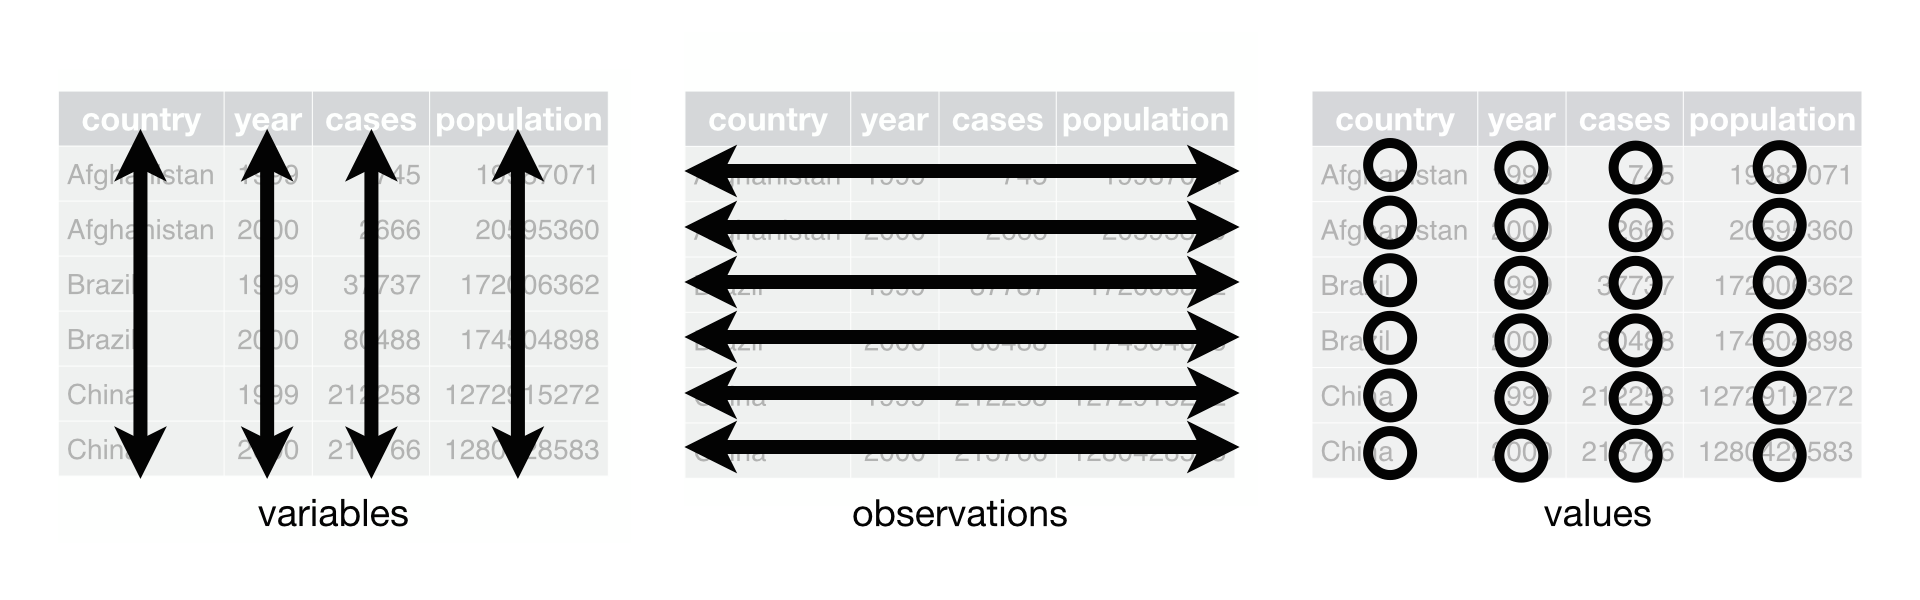
\includegraphics{tidy-1.png}
\caption{Figure 1: Components of a dataframe.}
\end{figure}

\hypertarget{creating-a-dataframe}{%
\subsection{Creating a dataframe}\label{creating-a-dataframe}}

\textbf{Syntax}

\begin{Shaded}
\begin{Highlighting}[]
\NormalTok{name_of_the_dataframe <-}\StringTok{ }\KeywordTok{data.frame}\NormalTok{(}
                          \DataTypeTok{var1_name=}\NormalTok{vector of values of the first variable,}
                          \DataTypeTok{var2_names=}\NormalTok{vector of values of the second variable)}
\end{Highlighting}
\end{Shaded}

\textbf{Example}

\begin{Shaded}
\begin{Highlighting}[]
\NormalTok{corona <-}\StringTok{ }\KeywordTok{data.frame}\NormalTok{(}\DataTypeTok{ID=}\KeywordTok{c}\NormalTok{(}\StringTok{"C001"}\NormalTok{, }\StringTok{"C002"}\NormalTok{, }\StringTok{"C003"}\NormalTok{, }\StringTok{"C004"}\NormalTok{),}
                     \DataTypeTok{Location=}\KeywordTok{c}\NormalTok{(}\StringTok{"Beijing"}\NormalTok{, }\StringTok{"Wuhan"}\NormalTok{, }\StringTok{"Shanghai"}\NormalTok{, }\StringTok{"Beijing"}\NormalTok{),}
                     \DataTypeTok{Test_Results=}\KeywordTok{c}\NormalTok{(}\OtherTok{FALSE}\NormalTok{, }\OtherTok{TRUE}\NormalTok{, }\OtherTok{FALSE}\NormalTok{, }\OtherTok{FALSE}\NormalTok{))}
\NormalTok{corona}
\end{Highlighting}
\end{Shaded}

\begin{verbatim}
    ID Location Test_Results
1 C001  Beijing        FALSE
2 C002    Wuhan         TRUE
3 C003 Shanghai        FALSE
4 C004  Beijing        FALSE
\end{verbatim}

To check if it is a datafrme

\begin{Shaded}
\begin{Highlighting}[]
\KeywordTok{is.data.frame}\NormalTok{(corona)}
\end{Highlighting}
\end{Shaded}

\begin{verbatim}
[1] TRUE
\end{verbatim}

To convert a matrix to a dataframe

\begin{Shaded}
\begin{Highlighting}[]
\NormalTok{mat <-}\StringTok{ }\KeywordTok{matrix}\NormalTok{(}\DecValTok{10}\OperatorTok{:}\DecValTok{81}\NormalTok{, }\DataTypeTok{ncol=}\DecValTok{4}\NormalTok{)}
\NormalTok{mat}
\end{Highlighting}
\end{Shaded}

\begin{verbatim}
      [,1] [,2] [,3] [,4]
 [1,]   10   28   46   64
 [2,]   11   29   47   65
 [3,]   12   30   48   66
 [4,]   13   31   49   67
 [5,]   14   32   50   68
 [6,]   15   33   51   69
 [7,]   16   34   52   70
 [8,]   17   35   53   71
 [9,]   18   36   54   72
[10,]   19   37   55   73
[11,]   20   38   56   74
[12,]   21   39   57   75
[13,]   22   40   58   76
[14,]   23   41   59   77
[15,]   24   42   60   78
[16,]   25   43   61   79
[17,]   26   44   62   80
[18,]   27   45   63   81
\end{verbatim}

\begin{Shaded}
\begin{Highlighting}[]
\NormalTok{mat_df <-}\StringTok{ }\KeywordTok{as.data.frame}\NormalTok{(mat)}
\NormalTok{mat_df}
\end{Highlighting}
\end{Shaded}

\begin{verbatim}
   V1 V2 V3 V4
1  10 28 46 64
2  11 29 47 65
3  12 30 48 66
4  13 31 49 67
5  14 32 50 68
6  15 33 51 69
7  16 34 52 70
8  17 35 53 71
9  18 36 54 72
10 19 37 55 73
11 20 38 56 74
12 21 39 57 75
13 22 40 58 76
14 23 41 59 77
15 24 42 60 78
16 25 43 61 79
17 26 44 62 80
18 27 45 63 81
\end{verbatim}

\hypertarget{subsetting-data-frames}{%
\subsection{Subsetting data frames}\label{subsetting-data-frames}}

\textbf{Select rows}

\begin{Shaded}
\begin{Highlighting}[]
\KeywordTok{head}\NormalTok{(mat_df) }\CommentTok{# default it shows 5 rows}
\end{Highlighting}
\end{Shaded}

\begin{verbatim}
  V1 V2 V3 V4
1 10 28 46 64
2 11 29 47 65
3 12 30 48 66
4 13 31 49 67
5 14 32 50 68
6 15 33 51 69
\end{verbatim}

\begin{Shaded}
\begin{Highlighting}[]
\KeywordTok{head}\NormalTok{(mat_df, }\DecValTok{3}\NormalTok{) }\CommentTok{# To extract only the first three rows }
\end{Highlighting}
\end{Shaded}

\begin{verbatim}
  V1 V2 V3 V4
1 10 28 46 64
2 11 29 47 65
3 12 30 48 66
\end{verbatim}

\begin{Shaded}
\begin{Highlighting}[]
\KeywordTok{tail}\NormalTok{(mat_df)}
\end{Highlighting}
\end{Shaded}

\begin{verbatim}
   V1 V2 V3 V4
13 22 40 58 76
14 23 41 59 77
15 24 42 60 78
16 25 43 61 79
17 26 44 62 80
18 27 45 63 81
\end{verbatim}

To select some specific rows

\begin{Shaded}
\begin{Highlighting}[]
\NormalTok{index <-}\StringTok{ }\KeywordTok{c}\NormalTok{(}\DecValTok{1}\NormalTok{, }\DecValTok{3}\NormalTok{, }\DecValTok{7}\NormalTok{, }\DecValTok{8}\NormalTok{)}
\NormalTok{mat_df[index, ]}
\end{Highlighting}
\end{Shaded}

\begin{verbatim}
  V1 V2 V3 V4
1 10 28 46 64
3 12 30 48 66
7 16 34 52 70
8 17 35 53 71
\end{verbatim}

\textbf{Select columns}

\begin{enumerate}
\def\labelenumi{\arabic{enumi}.}
\tightlist
\item
  Select column(s) by variable names
\end{enumerate}

\begin{Shaded}
\begin{Highlighting}[]
\NormalTok{mat_df}\OperatorTok{$}\NormalTok{V1 }\CommentTok{# Method 1}
\end{Highlighting}
\end{Shaded}

\begin{verbatim}
 [1] 10 11 12 13 14 15 16 17 18 19 20 21 22 23 24 25 26 27
\end{verbatim}

\begin{Shaded}
\begin{Highlighting}[]
\NormalTok{mat_df[, }\StringTok{"V1"}\NormalTok{] }\CommentTok{# Method 2}
\end{Highlighting}
\end{Shaded}

\begin{verbatim}
 [1] 10 11 12 13 14 15 16 17 18 19 20 21 22 23 24 25 26 27
\end{verbatim}

\begin{enumerate}
\def\labelenumi{\arabic{enumi}.}
\setcounter{enumi}{1}
\tightlist
\item
  Select column(s) by index
\end{enumerate}

\begin{Shaded}
\begin{Highlighting}[]
\NormalTok{mat_df[, }\DecValTok{2}\NormalTok{]}
\end{Highlighting}
\end{Shaded}

\begin{verbatim}
 [1] 28 29 30 31 32 33 34 35 36 37 38 39 40 41 42 43 44 45
\end{verbatim}

\hypertarget{built-in-dataframes}{%
\subsection{Built in dataframes}\label{built-in-dataframes}}

\textbf{Note:} All objects in R have a class.

\hypertarget{function}{%
\chapter{Functions in R}\label{function}}

A function is a block of organized and reusable code that is used to perform a specific task in a program. There are two types of functions in R:

\begin{enumerate}
\def\labelenumi{\arabic{enumi}.}
\item
  In-built functions
\item
  User-defined functions
\end{enumerate}

\hypertarget{in-built-functions}{%
\section{In-built functions}\label{in-built-functions}}

These functions in R programming are provided by R environment for direct execution, to make our work easier Some examples for the frequently used in-built functions are as follows.

\begin{Shaded}
\begin{Highlighting}[]
\KeywordTok{mean}\NormalTok{(}\KeywordTok{c}\NormalTok{(}\DecValTok{10}\NormalTok{, }\DecValTok{20}\NormalTok{, }\DecValTok{21}\NormalTok{, }\DecValTok{78}\NormalTok{, }\DecValTok{105}\NormalTok{))}
\end{Highlighting}
\end{Shaded}

\begin{verbatim}
[1] 46.8
\end{verbatim}

\hypertarget{user-defined-functions}{%
\section{User-defined functions}\label{user-defined-functions}}

These functions in R programming language are dclared and defined by a user according to the requirements, to perform a specific task.

\hypertarget{main-components-of-a-function}{%
\section{Main components of a function}\label{main-components-of-a-function}}

All R functions have three main components: (Check this with Hadley's book)

\begin{enumerate}
\def\labelenumi{\arabic{enumi}.}
\item
  \textbf{function name}: name of the function that is stored as an R object
\item
  \textbf{arguments:} are used to rovide specific inputs to a function while a function is invoked. A function can have zero, single, multiple or default arguments.
\item
  \textbf{function body:} contains the block of code that performs the specific task assigned to a function. \textbf{return value}
\end{enumerate}

\hypertarget{passing-arguments-to-a-function}{%
\section{Passing arguments to a function}\label{passing-arguments-to-a-function}}

\hypertarget{some-useful-built-in-functions-in-r}{%
\section{Some useful built-in functions in R}\label{some-useful-built-in-functions-in-r}}

\hypertarget{r-can-be-used-as-a-simple-calculator.}{%
\subsection{R can be used as a simple calculator.}\label{r-can-be-used-as-a-simple-calculator.}}

\begin{longtable}[]{@{}ll@{}}
\toprule
\begin{minipage}[b]{0.47\columnwidth}\raggedright
Operator\strut
\end{minipage} & \begin{minipage}[b]{0.47\columnwidth}\raggedright
Description\strut
\end{minipage}\tabularnewline
\midrule
\endhead
\begin{minipage}[t]{0.47\columnwidth}\raggedright
+\strut
\end{minipage} & \begin{minipage}[t]{0.47\columnwidth}\raggedright
addition\strut
\end{minipage}\tabularnewline
\begin{minipage}[t]{0.47\columnwidth}\raggedright
-\strut
\end{minipage} & \begin{minipage}[t]{0.47\columnwidth}\raggedright
substraction\strut
\end{minipage}\tabularnewline
\begin{minipage}[t]{0.47\columnwidth}\raggedright
*\strut
\end{minipage} & \begin{minipage}[t]{0.47\columnwidth}\raggedright
multiplication\strut
\end{minipage}\tabularnewline
\begin{minipage}[t]{0.47\columnwidth}\raggedright
\^{}\strut
\end{minipage} & \begin{minipage}[t]{0.47\columnwidth}\raggedright
exponentiation (5\^{}2 is 25)\strut
\end{minipage}\tabularnewline
\begin{minipage}[t]{0.47\columnwidth}\raggedright
\%\%\strut
\end{minipage} & \begin{minipage}[t]{0.47\columnwidth}\raggedright
modulo-remainder of the division of the number to the left by the number on its right. (5\%\%3 is 2)\strut
\end{minipage}\tabularnewline
\bottomrule
\end{longtable}

\hypertarget{some-more-maths-functions}{%
\subsection{Some more maths functions}\label{some-more-maths-functions}}

\begin{longtable}[]{@{}ll@{}}
\toprule
\begin{minipage}[b]{0.47\columnwidth}\raggedright
Operator\strut
\end{minipage} & \begin{minipage}[b]{0.47\columnwidth}\raggedright
Description\strut
\end{minipage}\tabularnewline
\midrule
\endhead
\begin{minipage}[t]{0.47\columnwidth}\raggedright
abs(x)\strut
\end{minipage} & \begin{minipage}[t]{0.47\columnwidth}\raggedright
absolute value of x\strut
\end{minipage}\tabularnewline
\begin{minipage}[t]{0.47\columnwidth}\raggedright
log(x, base=y)\strut
\end{minipage} & \begin{minipage}[t]{0.47\columnwidth}\raggedright
logarithm of x with base y; if base is not specified, returns the natural logarithm\strut
\end{minipage}\tabularnewline
\begin{minipage}[t]{0.47\columnwidth}\raggedright
exp(x)\strut
\end{minipage} & \begin{minipage}[t]{0.47\columnwidth}\raggedright
exponential of x\strut
\end{minipage}\tabularnewline
\begin{minipage}[t]{0.47\columnwidth}\raggedright
sqrt(x)\strut
\end{minipage} & \begin{minipage}[t]{0.47\columnwidth}\raggedright
square root of x\strut
\end{minipage}\tabularnewline
\begin{minipage}[t]{0.47\columnwidth}\raggedright
factorial(x)\strut
\end{minipage} & \begin{minipage}[t]{0.47\columnwidth}\raggedright
factorial of x\strut
\end{minipage}\tabularnewline
\bottomrule
\end{longtable}

\hypertarget{basic-statistic-functions}{%
\subsection{Basic statistic functions}\label{basic-statistic-functions}}

\begin{longtable}[]{@{}ll@{}}
\toprule
Operator & Description\tabularnewline
\midrule
\endhead
mean(x) & mean of x\tabularnewline
median(x) & median of x\tabularnewline
mode(x) & mode of x\tabularnewline
var(x) & variance of x\tabularnewline
scale(x) & z-score of x\tabularnewline
quantile(x) & quantiles of x\tabularnewline
summary(x) & summary of x: mean, minimum, maximum, etc.\tabularnewline
\bottomrule
\end{longtable}

\hypertarget{probability-distribution-functions}{%
\subsection{Probability distribution functions}\label{probability-distribution-functions}}

\begin{itemize}
\item
  \textbf{d} prefix for the \textbf{distribution} function
\item
  \textbf{p} prefix for the \textbf{cummulative probability}
\item
  \textbf{q} prefix for the \textbf{quantile}
\item
  \textbf{r} prefix for the \textbf{random} number generator
\end{itemize}

\hypertarget{illustration-with-standard-normal-distribution}{%
\subsubsection{Illustration with Standard normal distribution}\label{illustration-with-standard-normal-distribution}}

The general formula for the probability density function of the normal distribution with mean \(\mu\) and variance \(\sigma\) is given by

\[
f_X(x) = \frac{1}{\sigma\sqrt{(2\pi)}} e^{-(x-\mu)^2/2\sigma^2}
\]

If we let the mean \(\mu=0\) and the standard deviation \(\sigma=1\), we get the probability density function for the standard normal distribution.

\[
f_X(x) = \frac{1}{\sqrt{(2\pi)}} e^{-(x)^2/2}
\]

\begin{Shaded}
\begin{Highlighting}[]
\KeywordTok{dnorm}\NormalTok{(}\DecValTok{0}\NormalTok{)}
\end{Highlighting}
\end{Shaded}

\begin{verbatim}
[1] 0.3989423
\end{verbatim}

\begin{figure}
\centering
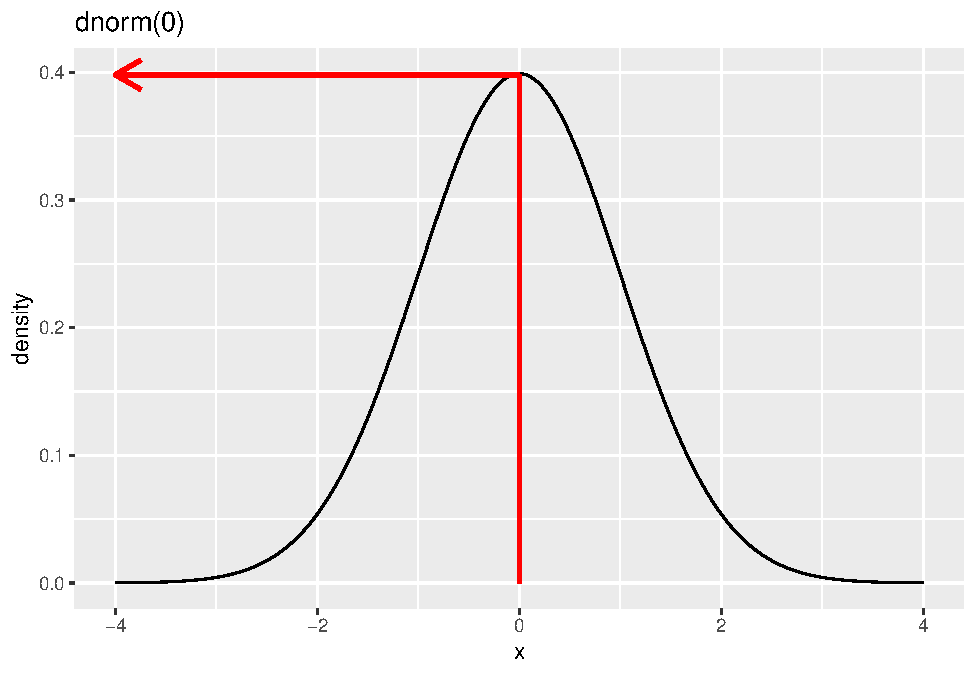
\includegraphics{STA-326-2.0-R-programming-and-Data-Analysis_files/figure-latex/unnamed-chunk-40-1.pdf}
\caption{\label{fig:unnamed-chunk-40}Standard normal probability density function: dnorm(0)}
\end{figure}

\begin{Shaded}
\begin{Highlighting}[]
\KeywordTok{pnorm}\NormalTok{(}\DecValTok{0}\NormalTok{)}
\end{Highlighting}
\end{Shaded}

\begin{verbatim}
[1] 0.5
\end{verbatim}

\begin{figure}
\centering
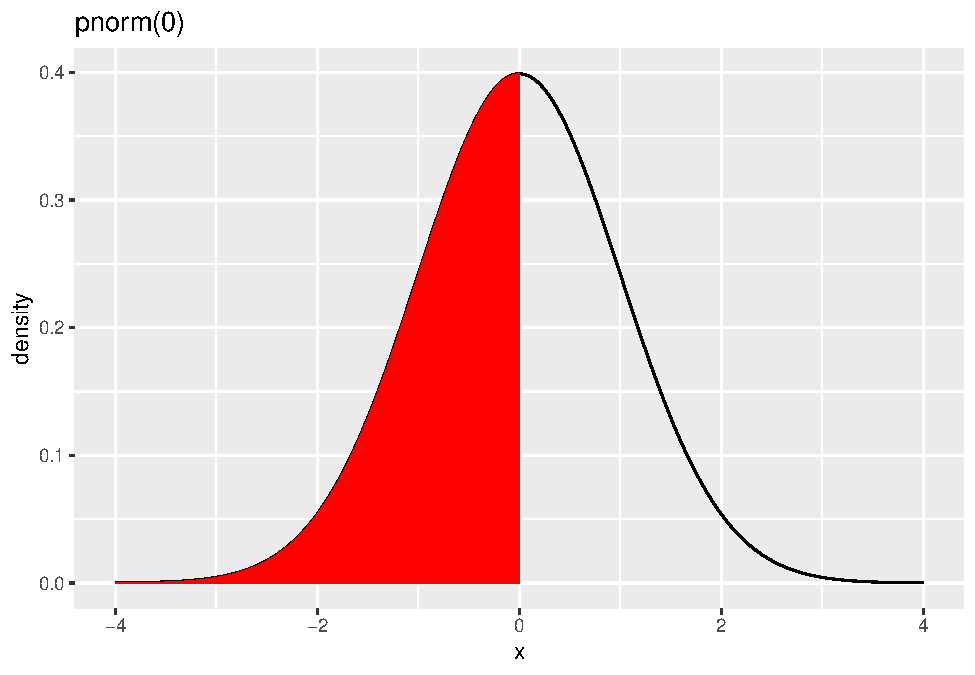
\includegraphics{STA-326-2.0-R-programming-and-Data-Analysis_files/figure-latex/unnamed-chunk-42-1.pdf}
\caption{\label{fig:unnamed-chunk-42}Standard normal probability density function: dnorm(0)}
\end{figure}

\begin{Shaded}
\begin{Highlighting}[]
\KeywordTok{qnorm}\NormalTok{(}\FloatTok{0.5}\NormalTok{)}
\end{Highlighting}
\end{Shaded}

\begin{verbatim}
[1] 0
\end{verbatim}

\begin{figure}
\centering
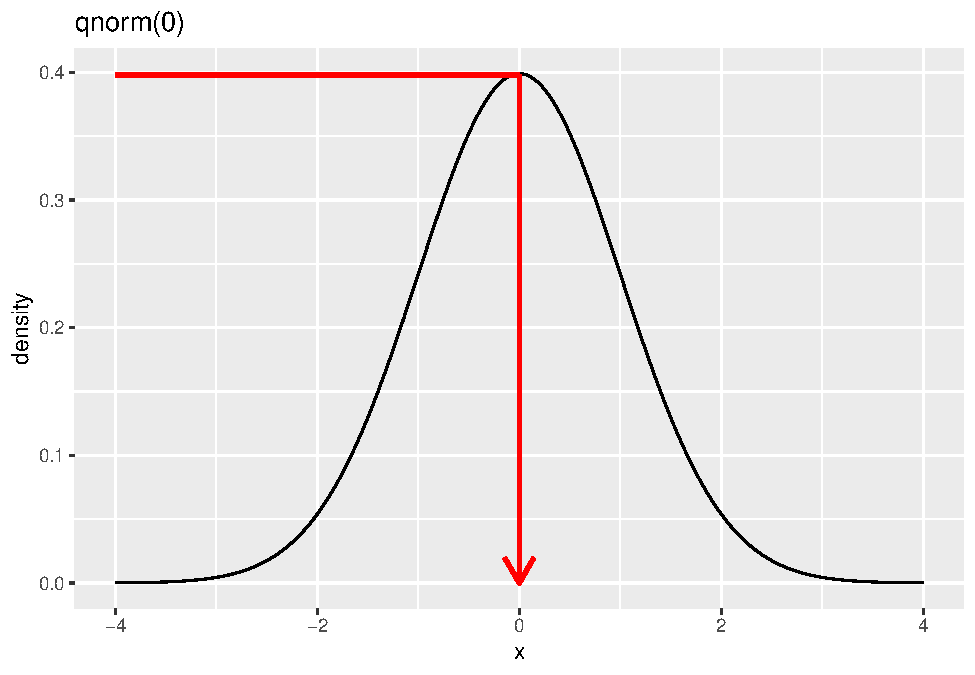
\includegraphics{STA-326-2.0-R-programming-and-Data-Analysis_files/figure-latex/unnamed-chunk-44-1.pdf}
\caption{\label{fig:unnamed-chunk-44}Standard normal probability density function: dnorm(0)}
\end{figure}

\begin{Shaded}
\begin{Highlighting}[]
\KeywordTok{set.seed}\NormalTok{(}\DecValTok{262020}\NormalTok{)}
\NormalTok{random_numbers <-}\StringTok{ }\KeywordTok{rnorm}\NormalTok{(}\DecValTok{10}\NormalTok{)}
\NormalTok{random_numbers}
\end{Highlighting}
\end{Shaded}

\begin{verbatim}
 [1]  0.20078181  0.95873346  1.18369056  1.49513750  1.18109222 -0.57789570
 [7]  0.01790671  0.81185245  0.39488199 -0.44337927
\end{verbatim}

\begin{Shaded}
\begin{Highlighting}[]
\KeywordTok{sort}\NormalTok{(random_numbers) }\CommentTok{## sort the numbers then it is easy to map with the graph}
\end{Highlighting}
\end{Shaded}

\begin{verbatim}
 [1] -0.57789570 -0.44337927  0.01790671  0.20078181  0.39488199  0.81185245
 [7]  0.95873346  1.18109222  1.18369056  1.49513750
\end{verbatim}

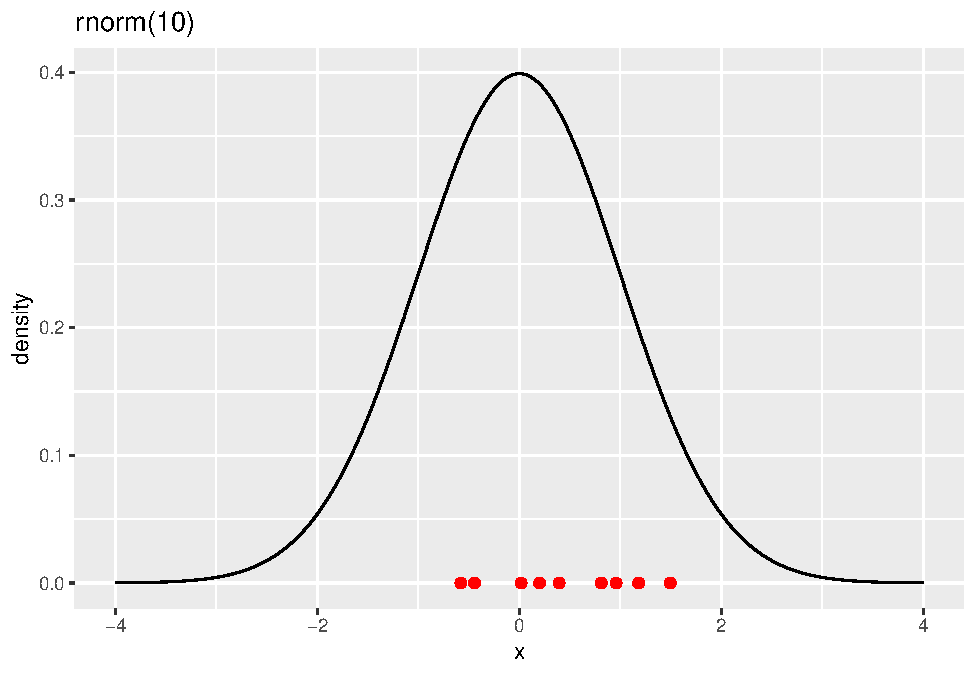
\includegraphics{STA-326-2.0-R-programming-and-Data-Analysis_files/figure-latex/unnamed-chunk-46-1.pdf}

\hypertarget{reproducibility-of-scientific-results}{%
\subsection{Reproducibility of scientific results}\label{reproducibility-of-scientific-results}}

\begin{Shaded}
\begin{Highlighting}[]
\KeywordTok{rnorm}\NormalTok{(}\DecValTok{10}\NormalTok{) }\CommentTok{# first attempt}
\end{Highlighting}
\end{Shaded}

\begin{verbatim}
 [1]  1.4701904 -0.2375662  0.1765985 -0.5257483 -1.3674764 -1.4422500
 [7]  0.7576607  0.6475122 -1.1543034  0.9066248
\end{verbatim}

\begin{Shaded}
\begin{Highlighting}[]
\KeywordTok{rnorm}\NormalTok{(}\DecValTok{10}\NormalTok{) }\CommentTok{# second attempt}
\end{Highlighting}
\end{Shaded}

\begin{verbatim}
 [1] -1.7603264 -0.3402939 -1.0335807  1.0645014 -0.3874459  0.5975271
 [7] -2.1535707  0.6602928  1.1581404  0.6133446
\end{verbatim}

As you can see above you will get different results

\begin{Shaded}
\begin{Highlighting}[]
\KeywordTok{set.seed}\NormalTok{(}\DecValTok{1}\NormalTok{)}
\KeywordTok{rnorm}\NormalTok{(}\DecValTok{10}\NormalTok{) }\CommentTok{# First attempt with set.seed}
\end{Highlighting}
\end{Shaded}

\begin{verbatim}
 [1] -0.6264538  0.1836433 -0.8356286  1.5952808  0.3295078 -0.8204684
 [7]  0.4874291  0.7383247  0.5757814 -0.3053884
\end{verbatim}

\begin{Shaded}
\begin{Highlighting}[]
\KeywordTok{set.seed}\NormalTok{(}\DecValTok{1}\NormalTok{)}
\KeywordTok{rnorm}\NormalTok{(}\DecValTok{10}\NormalTok{) }\CommentTok{# Second attempt with set.seed}
\end{Highlighting}
\end{Shaded}

\begin{verbatim}
 [1] -0.6264538  0.1836433 -0.8356286  1.5952808  0.3295078 -0.8204684
 [7]  0.4874291  0.7383247  0.5757814 -0.3053884
\end{verbatim}

\hypertarget{writing-functions}{%
\chapter{Writing functions}\label{writing-functions}}

\hypertarget{when-should-we-write-functions}{%
\section{When should we write functions?}\label{when-should-we-write-functions}}

\begin{itemize}
\tightlist
\item
  do many repetitive task
\end{itemize}

\hypertarget{glogal-variables-vs-local-variables}{%
\section{Glogal variables vs local variables}\label{glogal-variables-vs-local-variables}}

\hypertarget{control-structures}{%
\section{Control structures}\label{control-structures}}

\begin{itemize}
\tightlist
\item
  for loops
\end{itemize}

\hypertarget{lapply-apply..}{%
\section{lapply, apply..}\label{lapply-apply..}}

\hypertarget{data-analysis-with-tidyverse}{%
\chapter{Data analysis with tidyverse}\label{data-analysis-with-tidyverse}}

Some \emph{significant} applications are demonstrated in this chapter.

\hypertarget{tidy-data}{%
\section{Tidy data}\label{tidy-data}}

Two key principles:

\begin{enumerate}
\def\labelenumi{\arabic{enumi}.}
\item
  Put each dataset in a dataframe
\item
  Put each variable in a column
\end{enumerate}

\begin{figure}
\centering
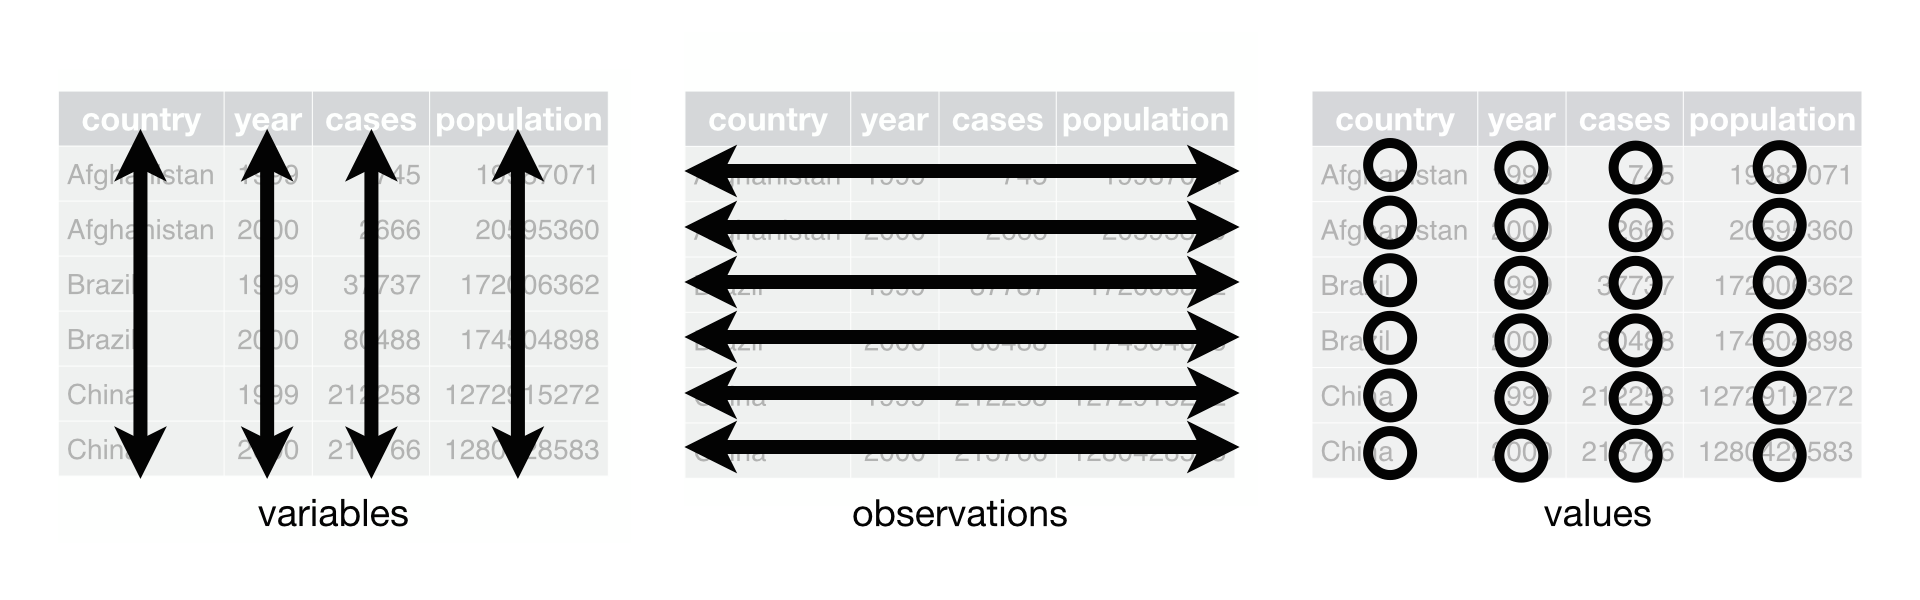
\includegraphics{tidy-1.png}
\caption{Figure 1: Components of a dataframe.}
\end{figure}

Vedio: \url{https://www.youtube.com/watch?v=K-ss_ag2k9E}

\hypertarget{convert-from-messy-data-to-tidy-data}{%
\subsection{Convert from messy data to tidy data}\label{convert-from-messy-data-to-tidy-data}}

``Tidy dataset are all alike; every messy dataset is messy in its own way.'' \_ Hadley Wickham

\hypertarget{data-wrangliing}{%
\chapter{Data wrangliing}\label{data-wrangliing}}

\hypertarget{data-visualisation}{%
\chapter{Data visualisation}\label{data-visualisation}}

\hypertarget{modelling}{%
\chapter{Modelling}\label{modelling}}

\hypertarget{simulation-based-inference}{%
\section{Simulation-based Inference}\label{simulation-based-inference}}

  \bibliography{book.bib,packages.bib}

\end{document}
